%----------------------------------------------------------------------------------------
%	PACKAGES AND DOCUMENT CONFIGURATIONS
%----------------------------------------------------------------------------------------
\documentclass[11pt]{article}
\usepackage{amsmath} % Required for some math elements
\usepackage{hyperref} 
\usepackage[usenames,dvipsnames]{xcolor}
\usepackage{lipsum} 
\usepackage{cite}
\usepackage{graphicx} % Required for the inclusion of images
\usepackage{algorithmic}
\usepackage{array}
\usepackage{bookmark}
\usepackage{listings}
\usepackage{amssymb}
\usepackage{enumitem}
\usepackage[margin=24mm]{geometry}
\usepackage[caption=false, font=footnotesize]{subfig}
\usepackage{multirow}
\usepackage[active,tightpage]{preview}

\renewcommand{\PreviewBorder}{1in}
\newcommand{\Newpage}{\end{preview}\begin{preview}}

\newlist{steps}{enumerate}{1}
\setlist[steps, 1]{label = Step \arabic*:}

\hypersetup{ %color attributes of citation, link, etc.
    colorlinks=true,
    linkcolor=blue,
    filecolor=gray,      
    urlcolor=blue,
    citecolor=blue,
}

 
\lstdefinelanguage{VHDL}{
   morekeywords=[1]{
     library,use,all,entity,is,port,in,out,end,architecture,of,
     begin,and,or,Not,downto,ALL
   },
   morekeywords=[2]{
     STD_LOGIC_VECTOR,STD_LOGIC,IEEE,STD_LOGIC_1164,
     NUMERIC_STD,STD_LOGIC_ARITH,STD_LOGIC_UNSIGNED,std_logic_vector,
     std_logic
   },
   morecomment=[l]--
}
\definecolor{keyword}{rgb}{0,0.3,0.7}
\definecolor{STD}{rgb}{0.9,0.0,0.7}
\definecolor{comment}{rgb}{0.0,0.6,0.1}

\lstdefinestyle{vhdl}{
   language     = VHDL,
   basicstyle   = \footnotesize\ttfamily,
   keywordstyle = [1]\color{keyword}\bfseries,
   keywordstyle = [2]\color{STD}\bfseries,
   commentstyle = \color{comment}
   breaklines=true,                % sets automatic line breaking
   tabsize=3		                   % sets default tabsize to 2 spaces
}


\newcommand{\matlab}{\textsc{Matlab }} %very important and totally necessary addition

\newcommand\Item[1][]{%
  \ifx\relax#1\relax  \item \else \item[#1] \fi
  \abovedisplayskip=0pt\abovedisplayshortskip=0pt~\vspace*{-\baselineskip}}
  %----------------------------------------------------------------------------------------
%	DOCUMENT INFORMATION
%----------------------------------------------------------------------------------------
 
\title{ECEN302 : Integrated Digital Electronics \\ Assignment 1 Submission}
\author{Daniel Eisen : 300447549}
\date{\today}

\begin{document}
\begin{preview}
\maketitle
%----------------------------------------------------------------------------------------
%	DOCUMENT CONTENT
%----------------------------------------------------------------------------------------
\begin{enumerate}
  \item \textbf{Look up the data sheet for the device we are using in the laboratory and then answer the following questions:}

  The device on the Nexys4 DDR and A7 boards if is the Artix-7 100T.
  \begin{enumerate}
    \item \textit{How many CLBs are there?}

    There are 7925 CLB's  (15850 logic slice pairs).
    
    \item \textit{How many I/O pins?}

    The max supported single ended I/O is 300, but on the CSG324 package there are \textbf{210} user  available I/O pins. 

    \item \textit{What I/O voltages can be accommodated and how is this configured?}

    1.2V, 1.5V, 1.8V, 2.5V and, 3.3V. These are selected by setting the IOSTANDARD in I/O planning or in the constraints file of your project.
    
    \item \textit{What is the physical footprint?}

    The CSG324 package is 15x15 mm.

    \item \textit{What does “speed grade” mean?}

    Xilinx defines the 'Speed Grade" of specifically FPGA devices to be a general indication of the timing performance of that device. These are specified as relative rating with a device family. Ie -1,-2,-3 etc from slowest to fastest.
    Each speed grade level represents around a 10-15\% performance difference.

  \end{enumerate}

  \item \textbf{With reference to the CLB:}
  \begin{enumerate}
    \item \textit{How is combinatorial logic typically implemented?}
    
    \item \textit{What is the main purpose of the flipflops/latches?}

    \item \textit{What is the carry chain and what is it used for?}

    \item \textit{What is the deference between a SLICEM and a SLICEL?}

    \item \textit{How are the CLBs connected to other CLBs?}

  \end{enumerate}

  \item \textbf{With regard to FPGA design:}
  \begin{enumerate}
    \item \textit{Describe the principle of pipelining and why it is often necessary?}
    
    \item \textit{Explain “setup” and “hold” timing?}

    \item \textit{What is metastability and what are the two main causes of it?}

    \item \textit{How do we typically deal with metastability?}

    \item \textit{Describe the difference between Mealy and Moore FSMs}

  \end{enumerate}

  \item \textbf{VHDL design. Compare and Add Circuit.}
  \lstinputlisting[language=VHDL]{../compare_add/compare_add.srcs/sources_1/new/comp_add.vhd}

  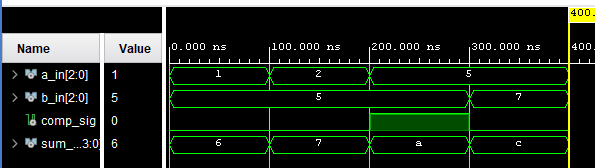
\includegraphics[width=\textwidth]{inc/sim.png}

  \lstinputlisting[language=VHDL]{../compare_add/compare_add.srcs/sim_1/new/comp_add_tb.vhd}
  

  \item \textbf{Below is a list of tools or methods that can assist and/or accelerate the development and debugging of code for FPGAs. For each one describe the process and its benefit to the developer. (note: it is expected that you write at least a quarter of an A4 page on each item. Feel free to include pictures).}
  \begin{enumerate}
    \item \textit{Schematic generation of synthesised and routed designs}
    \item \textit{Test bench simulation}
    \item \textit{Timing analyser}
    \item \textit{Integrated Logic Analyser (ILA)}
  \end{enumerate}



\end{enumerate}
\end{preview}
\end{document}